\newpage
\section{Aufgabe 1}
\subsection{Aufbau}
Die einzelnen Komponenten wurden auf ein Steckbrett aufgebracht und mit Kabeln und Steckverbindern miteinander verbunden. Die Spannungen \(U_{CE}\) und \(U_{BE}\) wurden jeweils mit dem Messgerät {\it Fluke 175} gemessen, die Ströme \(I_B\) und \(I_C\) jeweils mit dem Messgerät {\it Voltcraft VC220}. Aufgebaut wurde folgender Schaltplan:
\begin{center}
\begin{minipage}{\linewidth}
\centering
\makebox[0cm]{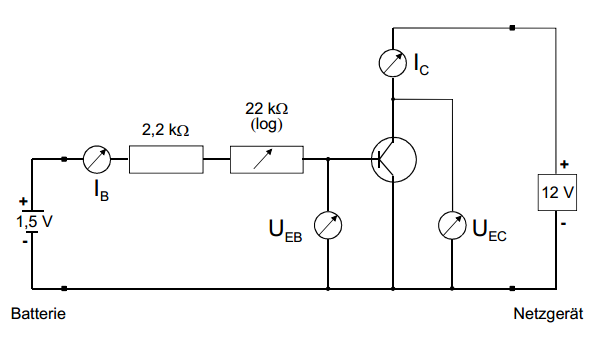
\includegraphics[width=\textwidth]{bilder/tra5}}
\captionof{figure}{Schaltplan für Aufgabe 1}%
\label{Schaltplan1}
\end{minipage}
\end{center}
Als Stromquelle für die Basis diente eine normale Batterie und für die Kollektorspannung ein regelbares \(12\, V\) Netzgerät. Alle anderen Komponenten wurden als Steckbrettkomponenten aus dem GP-Inventar in die Schaltung integriert.

\subsection{Fehlerabschätzung}
Als Grundlage für die Fehlerabschätzung werden die Herstellerangaben heran gezogen. Wie sich später zeigen wird, waren große systematische Fehler vorhanden, welche jedoch nicht mit der Gauß'schen Fehlerfortpflanzung betrachtet werden können. Benutzt wird daher: 
\begin{center}
\begin{tabular}{c|c|c|c}
Messgerät & Messgröße & Messbereich & Fehlerangabe \\\hline
Fluke 175 & \(U_{CE}\) & \(1\, V\) & \(0,8\% +3d\) \\
Fluke 175 & \(U_{CE}\) & \(1\, V\) & \(0,8\% +3d\) \\
Voltcraft VC220 & \(I_{B}\) & \(200 \, \mu A \) & \(\ 0,15\% +2d\) \\
Voltcraft VC220 & \(I_{C}\) & \(20 \, mA \) & \(\ 0,15\% +2d\)
\end{tabular}
\captionof{table}{Fehlerangaben von den Herstellern der Messgeräte}
\end{center}

\subsection{Durchführung}
Nachdem alle Geräte aufgebaut, eingeschaltet und eingestellt waren, wurde mit der Messung begonnen. Die Messung verlief von Anfang an äußerst durchwachsen. Das Messgerät, das \(I_B\) messen sollte, zeigte Werte in einer völlig falschen Größenordnung an und es war lange nicht klar, was die Ursache dafür war. Erst nach langen testen und einem kompletten Neuaufbau der Schaltung stellten wir fest, dass das Messgerät selber offensichtlich falsche Werte anzeigte. Das Messgerät wurde noch vor dem ersten notierten Wert getauscht. Nachdem das erledigt war, wurde mit der Aufnahme von Messwerten begonnen. Die Spannung \(U_{CE}\) wurde dabei bei jeder Messung um ca. \(1\,V\) erhöht, gestartet wurde bei einer Spannung von ca. \(1,2\,V\). Schon bei der Spannung \(U_{CE} \approx 6\,V\) zeigte das Messgerät für \(U_{BE}\) keine Spannung mehr an und es wurde durch ein identisches ersetzt. Dennoch zeigte sich gleich, dass der Messwert der beiden Geräte nicht gleich war. 

Aufgrund des immensen Zeitverlustes beim Aufbau für diese Aufgabe entschieden wir uns dafür nicht wie gedacht die Messwerte sofort skizzenhaft aufzuzeichnen, sondern achteten nur darauf, dass die Leistung des Transistors 
\(P = U_{CE} \cdot I_C \) nicht das Kritische Maß von \(2\,W\) überstieg. Die Messung wurde jeweils für Basisströme 
\(I_B = 30 \mu A, 60 \mu A, 90 \mu A, 120 \mu A\) durchgeführt.

\subsection{Beobachtung}
Zu beobachten war, dass die Spannung \(U_{BE}\) bei Variation von \(U_{CE}\) keines wegs konstant blieb, die Änderungen waren jedoch relativ klein. Bei der Messung von \(I_{C}\) war auch schon schnell zu sehen, dass die Messung nicht unseren Erwartungen entsprach, da die Werte sehr stark schwankten.

\subsection{Messwerte}
\begin{center}
\begin{tabular}{c|c|c|c}
\(I_B\) in \(\mu A\) & \(I_C\) in \(mA\) & \(U_{BE}\) in \(V\) & \(U_{CE}\) in \(V\) \\ \hline
\(29.9\) & \(3.83\) & \(0.706\) & \(1.218\) \\ 
\(29.9\) & \(3.86\) & \(0.706\) & \(2.015\) \\ 
\(29.9\) & \(3.89\) & \(0.705\) & \(3.005\) \\ 
\(30.2\) & \(3.73\) & \(0.697\) & \(4.086\) \\ 
\(30.7\) & \(3.53\) & \(0.685\) & \(5.005\) \\ 
\(31.0\) & \(3.51\) & \(0.557\) & \(6.031\) \\ 
\(36.2\) & \(3.16\) & \(0.557\) & \(6.96\) \\ 
\(36.0\) & \(3.21\) & \(0.542\) & \(8.02\) \\ 
\(38.0\) & \(3.16\) & \(0.492\) & \(9.05\) \\ 
\(39.5\) & \(3.14\) & \(0.445\) & \(10.04\) \\ 
\(41.4\) & \(3.15\) & \(0.390\) & \(11.01\) \\ 
\(34.9\) & \(3.15\) & \(0.352\) & \(12.04\)
\end{tabular}
\captionof{table}{Rohmesswerte vom statischen Kennlinienfeld bei \(I_B \approx 30 \mu A\)}
\vspace{0.4cm}

\begin{tabular}{c|c|c|c}
\(I_B\) in \(\mu A\) & \(I_C\) in \(mA\) & \(U_{BE}\) in \(V\) & \(U_{CE}\) in \(V\) \\ \hline
\(61.4\) & \(9.65\) & \(0.726\) & \(1.157\) \\ 
\(64.5\) & \(7.52\) & \(0.688\) & \(2.019\) \\ 
\(67.6\) & \(7.4\) & \(0.652\) & \(3.051\) \\ 
\(61.4\) & \(10.73\) & \(0.725\) & \(3.973\) \\ 
\(61.8\) & \(10.97\) & \(0.721\) & \(5.011\) \\ 
\(61.9\) & \(11.12\) & \(0.718\) & \(6.007\) \\ 
\(62.1\) & \(11.26\) & \(0.716\) & \(6.96\) \\ 
\(62.3\) & \(11.46\) & \(0.712\) & \(8.09\) \\ 
\(62.7\) & \(11.64\) & \(0.71\) & \(8.98\) \\ 
\(62.9\) & \(11.86\) & \(0.705\) & \(10.01\) \\ 
\(63.1\) & \(12.04\) & \(0.702\) & \(11.02\) \\ 
\(63.5\) & \(12.17\) & \(0.702\) & \(12.04\)
\end{tabular}
\captionof{table}{Rohmesswerte vom statischen Kennlinienfeld bei \(I_B \approx 60 \mu A\)}
\vspace{0.35cm}

\begin{tabular}{c|c|c|c}
\(I_B\) in \(\mu A\) & \(I_C\) in \(mA\) & \(U_{BE}\) in \(V\) & \(U_{CE}\) in \(V\) \\ \hline
\( 88.4\) & \(15\) & \(0.738\) & \(1.1\) \\ 
\(88.4\) & \(14.94\) & \(0.741\) & \(2.097\) \\ 
\(88.4\) & \(15.03\) & \(0.741\) & \(2.967\) \\ 
\(88.8\) & \(15.26\) & \(0.739\) & \(3.945\) \\ 
\(89.9\) & \(14.65\) & \(0.731\) & \(5.02\) \\ 
\(93.3\) & \(11.91\) & \(0.7\) & \(6.643\) \\ 
\(95.3\) & \(11.72\) & \(0.688\) & \(7.03\) \\ 
\(98.3\) & \(10.58\) & \(0.652\) & \(8.16\) \\ 
\(99.9\) & \(10.5\) & \(0.643\) & \(9.06\) \\ 
\(102.0\) & \(10.51\) & \(0.627\) & \(10.01\) \\ 
\(105.0\) & \(10.55\) & \(0.601\) & \(11.06\) \\ 
\(105.5\) & \(10.66\) & \(0.59\) & \(12.00 \)
\end{tabular}
\captionof{table}{Rohmesswerte vom statischen Kennlinienfeld bei \(I_B \approx 90 \mu A\)}
\vspace{0.35cm}

\begin{tabular}{c|c|c|c}
\(I_B\) in \(\mu A\) & \(I_C\) in \(mA\) & \(U_{BE}\) in \(V\) & \(U_{CE}\) in \(V\) \\ \hline
\( 118.3\) & \(19.43\) & \(0.751\) & \(1.053\) \\ 
\(118.8\) & \(19.95\) & \(0.747\) & \(2.048\) \\ 
\(119.3\) & \(20.4\) & \(0.743\) & \(3.112\) \\ 
\(120\) & \(20.7\) & \(0.739\) & \(4.027\) \\ 
\(122.8\) & \(18.8\) & \(0.721\) & \(5.088\) \\ 
\(125.4\) & \(16.2\) & \(0.702\) & \(6.095\) \\ 
\(129.4\) & \(14.2\) & \(0.672\) & \(7.24\) \\ 
\(133.0\) & \(13.7\) & \(0.658\) & \(8.006\) \\ 
\(134.8\) & \(13.8\) & \(0.65\) & \(9.03\) \\ 
\(136.8\) & \(13.7\) & \(0.635\) & \(10.18\) \\ 
\(140\) & \(13.8\) & \(0.621\) & \(11.07\) \\ 
\(140.8\) & \(13.9\) & \(0.61\) & \(12.08 \)
\end{tabular}
\captionof{table}{Rohmesswerte vom statischen Kennlinienfeld bei \(I_B \approx 120 \mu A\)}
\vspace{0.35cm}
\end{center}
\subsection{Das statische Kennlinienfeld}
Um die Daten im Rahmen der Aufgabe 1 auswerten zu können, werden die Messwerte in ein Kennlinienfeld eingetragen. Dabei werden im 1. und 4. Quadranten alle Messwerte verwendet, im 2. und 3. dagegen nur die, mit einer Kollektorsoannung von \(U_{CE} \approx 12\,V \). Um den Anstieg des als linear angenommenen Verlaufs der Werte im 2. Quadranten zu bestimmen, wurde die lineare Regression mit Fehler aus der Streuung verwendet. Das von GNU-Plot gelieferte Ergebnis ist:
\begin{equation}
m = 110 \pm 17
\end{equation}
\begin{center}
\begin{minipage}{\linewidth}
\centering
\makebox[0cm]{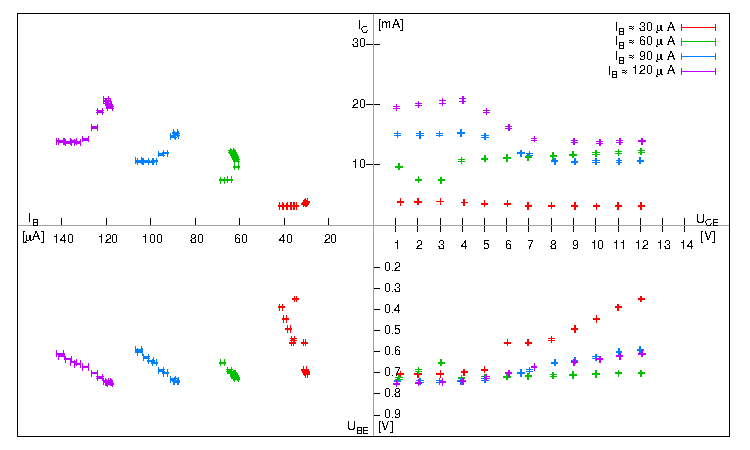
\includegraphics[width=20cm]{graphen/curve0}}
\captionof{figure}{Gemessenes Kennlinienfeld}%
\label{gnuplot_kennlinienfeld}
\end{minipage}
\end{center}
<<<<<<< HEAD
\subsection{Auswertung}
\subsubsection{erster Quadrant}
Durch Vergleich mit dem idealisiertem Transistor in Abbildung \ref{kennlinienfeld} wird deutlich, dass der Verlauf von \(I_C\) auf \(U_{CE}\) nicht den Erwartungen entspricht. Der Strom bei den Messungen mit \(I_B \approx 90 \mu A\) und \(I_B \approx 120 \mu A\) bricht ab einer Kollektorspannung von \(U_{CE} \approx 5\, V\) ein. Außerdem zeigt auch der Verlauf mit \(I_B \approx 60 \mu A\) zwei Ausreißer und der mit \(I_B \approx 30 \mu A\) faellt ab, obwohl \(I_C\) mit steigedenem \(U_{CE}\) steigen sollte.
\subsubsection{zweiter Quadrant}
Die Ermittelte Steigung \(m\) entspricht genau dem Verstärkungsfaktor \(\beta = \frac{I_C}{I_B}\) daher ist der Gemessene Wert:
=======

\subsection{Auswertung}
\subsubsection{Erster Quadrant}
Durch Vergleich mit dem idealisierten Transistor in Abbildung \ref{kennlinienfeld} wird deutlich, dass der Verlauf von \(I_C\) auf \(U_{CE}\) nicht den Erwartungen entspricht. Der Strom bei den Messungen mit \(I_B \approx 90 \mu A\) und \(I_B \approx 120 \mu A\) bricht ab einer Kollektorspannung von \(U_{CE} \approx 5\, V\) ein. Ausserdem zeigt auch der Verlauf mit \(I_B \approx 60 \mu A\) zwei Ausreißer und der mit \(I_B \approx 30 \mu A\) fällt ab, obwohl \(I_C\) mit steigendem \(U_{CE}\) eigentlich ansteigen sollte.

\subsubsection{Zweiter Quadrant}
Die ermittelte Steigung \(m\) entspricht genau dem Verstärkungsfaktor \(\beta = \frac{I_C}{I_B}\), daher ist der Gemessene Wert:
>>>>>>> a799fdf2e3444e595f0061b2459ddd52e8b6b747
\begin{equation}
\beta = m = 110 \pm 17 \notag
\end{equation}
Da nur Werte für 4 verschiedene \(I_{B}\) aufgenommen wurden ist die Bestimmung vom Verstärkungsfaktor recht unsicher. Außerdem ist auch offensichtlich, dass bei der Messung mit \(I_B \approx 60 \mu A\) etwas anders gelaufen ist als bei den anderen Basisströmen; Der Wert ist ein Ausreißer.
\subsubsection{Dritter Quadrant}
Wie auch schon im 1. und 2. Quadranten zeigt der gemessene Wert bei \(I_B \approx 60 \mu A\) einen Ausreißer. Ob der Verlauf der Kurve ansonsten der idealisierten Kurve entspricht lässt sich nicht sagen, da nur 4 Messwerte vorhanden sind.  

Um Werte für \(r_{EB}\) zu erhalten werden die drei Differenzen von \(U_{BE}\) und \(I_{B}\) genutzt, da im allgemeinen dieser Widerstand in diesem Fall nicht konstant ist.
\begin{center}
\begin{tabular}{c|c|c}
\(\Delta U_{BE}\, [\mu A]\) & \(\Delta I_B\, [V]\) &  \(r_{EB}\, [\Omega]\) \\\hline
34,9 - 63,5 & 0,352 - 0,702 & 13200\\
63,5 -104,5 & 0,702 - 0,59 & 2670\\
104,5 - 140,8 & 0,59 - 0,61 & 567
\end{tabular}
\captionof{table}{Werte fuer \(r_{EB}\)}
\end{center}
dabei wurde \(r_{EB}\)berechnet wie:
\begin{equation}
r_{EB} = \frac{U_{BE_1}-U_{BE_2}}{I_{B_1}-I_{B_2}}
\end{equation}

\subsubsection{Vierter Quadrant}
Der Verlauf der Kurven entspricht im Allgemeinen den Erwartungen. Das die Kurve ansteigen hat damit zu tun, dass bei realen Transistoren immer auch ein Teil der Kollektorspannung über die Basis abfließt. Der Sprung von \(U_{BE}\) bei der Messung mit \(I_B \approx 30 \mu A\) ist ziemlich eindeutig auf den Tausch des Messgeräts zurückzuführen.

\subsection{Fazit}
Es ist offensichtlich, dass die Messung nicht gut verlaufen ist. Die Messwerte haben Unstetigkeiten, was auf eine Fehleranfällige Schaltung hindeutet. Ausgelöst könnte das z.B. durch einen Wackelkontakt geworden sein. Erstaunlich ist auch, dass das eingewechselte Messgerät einen deutlich abweichenden Wert anzeigte. Es ist durchaus möglich, dass bei zu niedriger Batteriespannung auch schon vor dem kompletten Ausfall keine richtigen Messwerte angezeigt wurden, denn die Abweichung lag nicht in der angegebenen Fehlertoleranz. Die ermittelten Ergebnisse sind daher mit äußerster Vorsicht zu genießen und sollten nicht als Vergleichswerte herangezogen werden. 

Der Stromverstärkungsfaktor wurde bestimmt zu:
\begin{equation}
\beta = m = 110 \pm 20 \notag
\end{equation}

als Abschätzung für \(r_{EB}\) konnten folgende Werte ermittelt werden:

\begin{center}
\begin{tabular}{c|c|c}
\(\Delta U_{BE}\, [\mu A]\) & \(\Delta I_B\, [V]\) &  \(r_{EB}\, [\Omega]\) \\\hline
34,9 - 63,5 & 0,352 - 0,702 & 13200\\
63,5 -104,5 & 0,702 - 0,59 & 2670\\
104,5 - 140,8 & 0,59 - 0,61 & 567
\end{tabular}
<<<<<<< HEAD
\captionof{table}{Werte für \(r_{EB}\)}
\end{center}
=======
\captionof{table}{Werte fuer \(r_{EB}\)}
\end{center}
>>>>>>> a799fdf2e3444e595f0061b2459ddd52e8b6b747
